\begin{flushright} {\tiny {\color{gray} \tt pair\_qqq.tex}} \end{flushright}
%~~~~~~~~~~~~~~~~~~~~~~~~~~~~~~~~~~~~~~~~~~~~~~~~~~~~~~~~~~~~~~~~~~~~~~~~~~~~~~~~~~~~~~~~~~~~~~~~~~

This element pair is introduced in \textcite{zhan09} (2009).
In \textcite{huzh11} (2011) we find the following enlightening figure::
\begin{center}
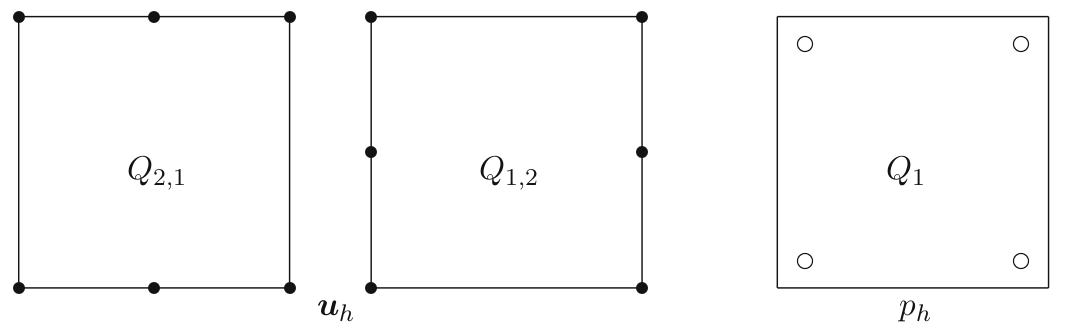
\includegraphics[width=8cm]{images/pair_qqq/huzh11}
\end{center}

The $u$-space basis functions are given by 
\[
\vec\bN_u = Q_2 \times Q_1 =
\left(
\begin{array}{c}
\frac12 r(r-1) \\
1-r^2 \\
\frac12 r(r+1)
\end{array}
\right)
\times
\left(
\frac12 (1-s) \qquad \frac12(1+s)
\right)
=
\left(
\begin{array}{c}
\frac12 r(r-1)  \frac12(1-s)\\ 
(1-r^2)         \frac12(1-s)\\
\frac12 r(r+1)  \frac12(1-s)\\
\frac12 r(r-1)  \frac12(1+s)\\
(1-r^2)         \frac12(1+s)\\
\frac12 r(r+1)  \frac12(1+s)
\end{array}
\right)
\]

\[
\vec\bN_v = Q_1 \times Q_2 = 
\left(
\begin{array}{c}
\frac12 (1-r) \\
\frac12(1+r)
\end{array}
\right)
\times
\left(
\frac12 s(s-1)  \quad
1-s^2 \quad
\frac12 s(s+1)
\right)
=
\left(
\begin{array}{c}
\frac12 (1-r) \frac12 s(s-1) \\
\frac12(1+r)  \frac12 s(s-1) \\
\frac12 (1-r) (1-s^2) \\
\frac12(1+r)  (1-s^2) \\
\frac12 (1-r) \frac12 s(s+1)\\
\frac12(1+r)  \frac12 s(s+1)
\end{array}
\right)
\]
The $u$-dofs and $v$-dofs are living on different nodes.
Based on the vectors above the numbering is then 
\begin{verbatim}
4===5===6   5=======6   4=======3
|       |   |       |   |       |
|       |   3       4   |       |
|       |   |       |   |       |
1===2===3   1=======2   1=======2

 u dofs      v dofs       p dofs

\end{verbatim}
In total, there are 6 $u$-dofs, 6 $v$-dofs and 4 $p$-dofs per element.

